\chapter{Application expérimentale}

\index{résultats}
\section{Viscosité}
Les résultats des mesures des réponses fréquentielles dans les quatre milieux sont présentés sur deux graphiques. Le premier, la figure \ref{fig:Réponse frequencielle amplitude}, représente l’amplitude du signal retourné par le capteur. Il semble que les amplitudes maximales varient selon une loi exponentielle. On remarque également que la partie gauche des courbes est partagée par l’ensemble des milieux. D’après ces premières observations, il semblerait que l’amplitude soit une variable dépendante de la fréquence de résonance, bien que cela ne puisse pas encore être affirmé avec certitude.

Le second graphe de la réponse fréquentielle est présenté dans la figure \ref{fig:Réponse frequencielle déphasage}. Les signaux y apparaissent très différents de ceux de l’amplitude. Notamment, l’eau et l’éthanol sont beaucoup plus proches de l’air que dans le graphique de l’amplitude. De plus, les maxima semblent être alignés. Une régression linéaire a été effectuée pour le vérifier, et en effet, il semble que les points soient alignés.


\begin{figure}[H]
    \centering
    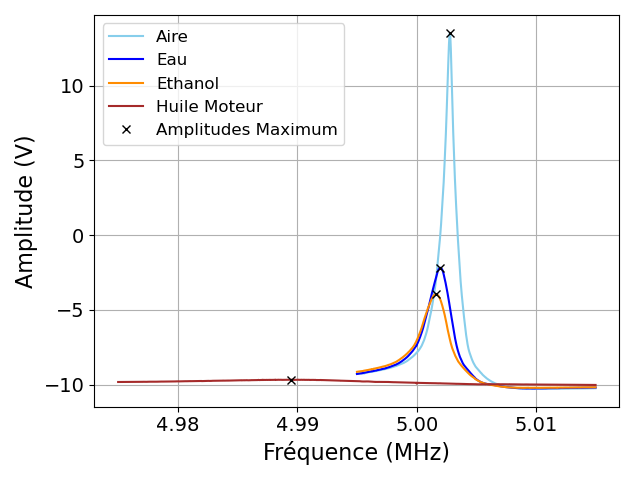
\includegraphics[width=0.8\textwidth]{assets/figures/reponseFrequence.png}
    \caption{Réponse fréquentielle en amplitude du capteur selon différents milieux}
    \label{fig:Réponse frequencielle amplitude}
\end{figure}

\begin{figure}[H]
    \centering
    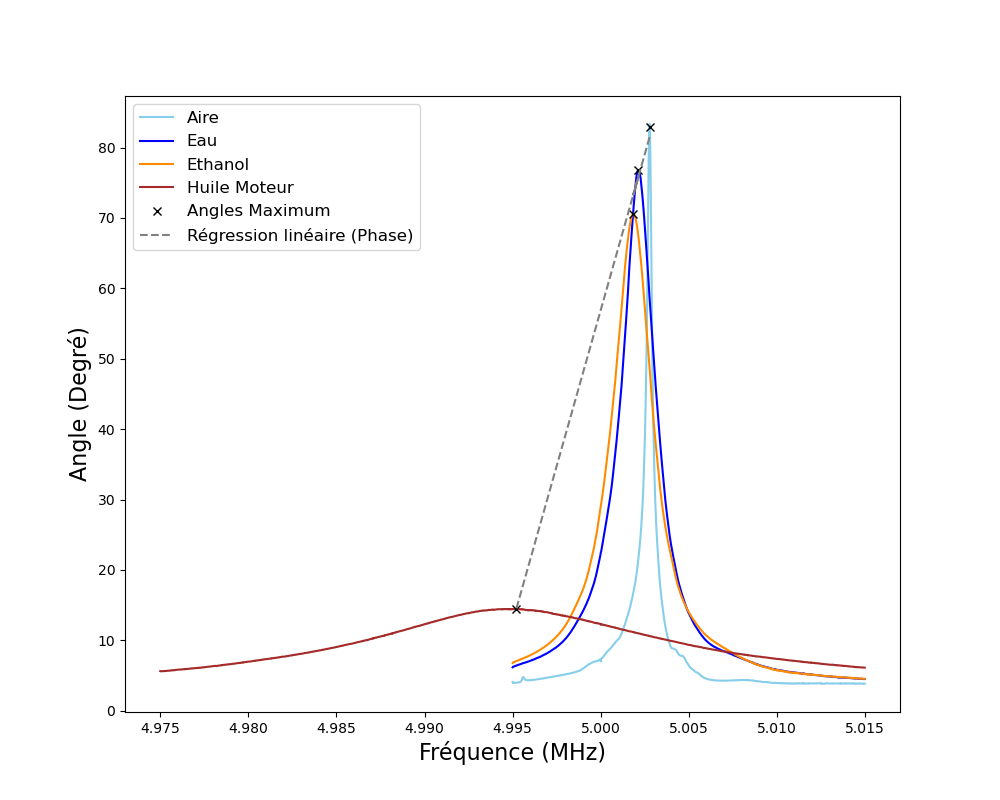
\includegraphics[width=0.8\textwidth]{assets/figures/reponsePhase.png}
    \caption{Réponse fréquentielle en phase du capteur selon différents milieux}
    \label{fig:Réponse frequencielle déphasage}
\end{figure}

\subsection{Discussion des résultats}
D’après les derniers résultats, il n’est pas encore possible de déterminer précisément la fonction qui relie la viscosité à l’amplitude. En revanche, il semble que les deux variables soient liées.
La figure \ref{fig:Viscosité des différents échantillons} présente la viscosité des différents échantillons mesurés à température ambiante, ainsi que l’amplitude de la résonance.
On observe que l’amplitude fréquentielle diminue avec l’augmentation de la viscosité des échantillons, ce qui est cohérent : plus le milieu est visqueux, plus il est difficile pour les ondes de se propager.
La figure \ref{fig:Amplitude VS Viscosité} montre l’amplitude de la résonance en fonction de la viscosité des différents échantillons.
Avec si peu de points, il n’est pas possible de déterminer une fonction exacte liant les deux variables. Les données suggèrent toutefois que la relation n’est pas linéaire.

Ne connaissant ni la marque ni le modèle de l’huile moteur utilisée, il est difficile de comparer précisément les résultats. La valeur de viscosité utilisée pour l’huile moteur n’est probablement pas exactement la même que celle fournie dans le Formulaire et table \cite{crm_viscosity_table}.
Pour les autres échantillons — l’eau, l’éthanol et l’air — les données sont cohérentes avec les valeurs attendues.
Cependant, la viscosité varie sensiblement en fonction de la température. Or, les mesures d’amplitude ont été effectuées à température ambiante, ce qui fausse également la comparaison avec les données théoriques.

\begin{figure}[H]
    \centering
    \begin{minipage}{0.48\textwidth}
        \centering
        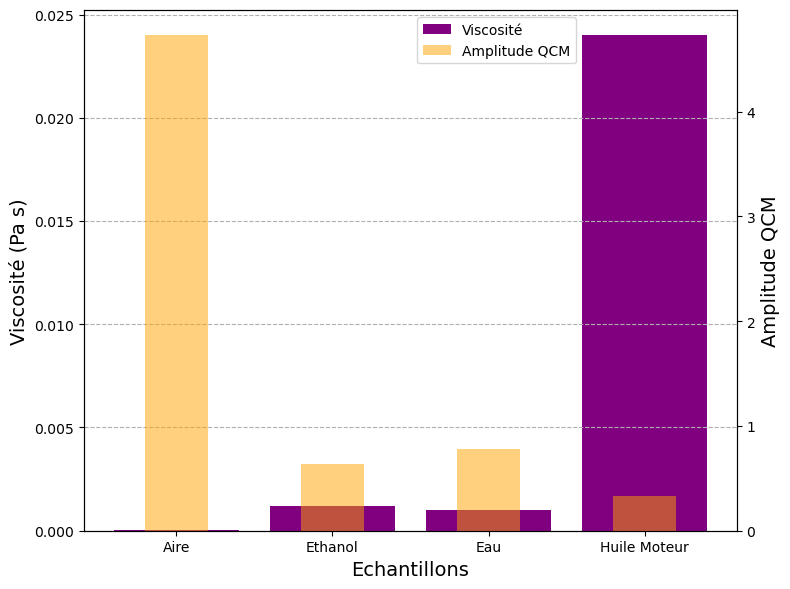
\includegraphics[width=\textwidth]{assets/figures/viscositeAmplitudeBar.png}
        \caption{Viscosité des différents échantillons mesurés à température ambiante et l'amplitude de la résonance}
        \label{fig:Viscosité des différents échantillons}
    \end{minipage}\hfill
    \begin{minipage}{0.48\textwidth}
        \centering
        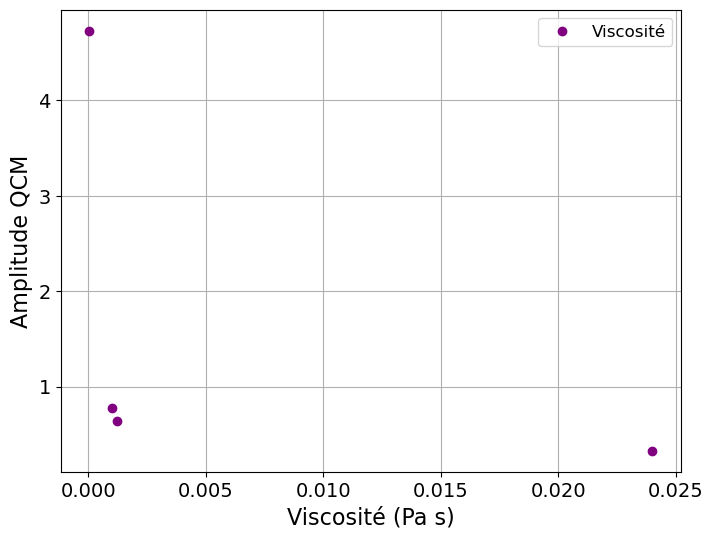
\includegraphics[width=\textwidth]{assets/figures/AmpitudeVSViscosite.png}
        \caption{Amplitude de la résonance en fonction de la viscosité des différents échantillons}
        \label{fig:Amplitude VS Viscosité}
    \end{minipage}
\end{figure}

\section{Gelification}
Les resultat de la mesure de la gelification sont présentés dans la figure \ref{fig:Frequence gelification}. 
Lorsque le liquide est refroidi,
un chagement de la pente entre de la fréquence de résonance et la température est visible au environ des 25°C, 
en dessus de cette temperature la pente est similaire à celle de l'eau. en dessous la pente est plus importante.  
Ce changement indiquerais un changement de l'état du gel. Passant de l'état liquide à l'état gélifié.
Une fois que le liquide à attein ca temérature minimal et que de l'eau chaude circule autour du capteur,
la temperature augment plus vite que la fréquance de raisonnance. un autre point de chacngement de phase est visible au environ de 32°C ce qui corrresponderais à la temperature de liquefaction de la gélatine en liquide.
\begin{figure}[H]
    \centering
    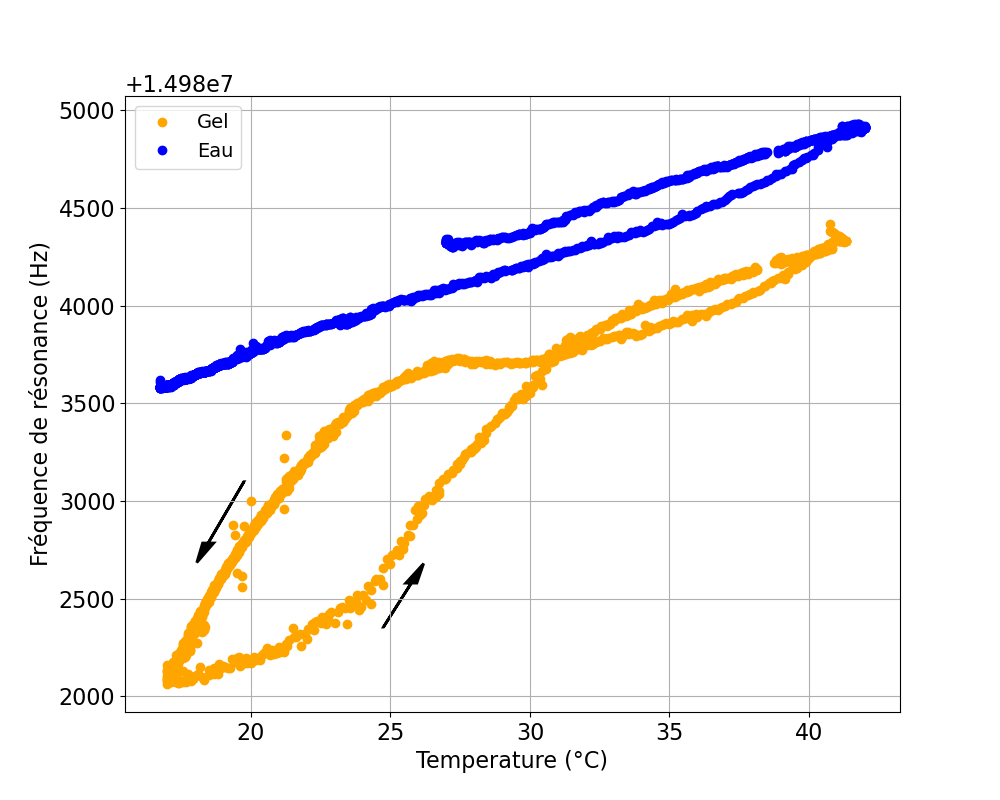
\includegraphics[width=0.8\textwidth]{assets/figures/gel.png}
    \caption{Frequence de résonance en fonction de la temperature pour la mesure de la gelification}
    \label{fig:Frequence gelification}
\end{figure}
\subsection{Discussion des résultats}
En comparant avec les données de la littérature \cite{SHA2019163}, la température de gélification varie entre 5 °C et 20 °C, tandis que la température de fusion se situe entre 20 °C et 30 °C. En effet, la température d’extraction, parmi d’autres variables, a un impact sur la température de solidification.

Les températures mesurées avec la microbalance à quartz présentent un léger écart par rapport aux données de la littérature. Cela pourrait s’expliquer par la position du capteur de température : en effet, ce dernier est situé sur un PCB, en dessous du quartz, ce qui entraîne un décalage avec la température réelle à l’intérieur du récipient. Cette différence pourrait donc justifier l’écart observé.


